\documentclass{article}
\usepackage[T1]{fontenc}
\usepackage{lmodern}
\usepackage{graphicx}
\usepackage{amsmath,amssymb}
\usepackage[a4paper,margin=2cm]{geometry}
\usepackage[absolute,overlay]{textpos}
\setlength{\TPHorizModule}{1mm}
\setlength{\TPVertModule}{1mm}
\usepackage[indonesian]{babel}
\usepackage{hyperref}
\setlength{\emergencystretch}{2em}
% unit: Halaman 51

\begin{document}

% === Halaman 51 (llm) ===

\begin{itemize}
    \item Secara intuitif: jika jarak antara dua buah \textit{string} yang berulang di dalam plainteks merupakan kelipatan dari panjang kunci,
    \item maka \textit{string} yang sama tersebut akan muncul menjadi kriptogram yang sama pula di dalam cipherteks.
    \item Pada Contoh 1,
    \begin{itemize}
        \item kunci = \texttt{abcd}
        \item panjang kunci = 4
        \item jarak antara dua \texttt{crypto} yang berulang = 16
        \item $16 = \text{kelipatan } 4$
    \end{itemize}
\end{itemize}

\vspace{10mm}

$\therefore$ \texttt{crypto} dienkripsi menjadi kriptogram yang sama

% deskripsi: Ilustrasi proses enkripsi Vigenere cipher yang menunjukkan plainteks 'cryptoisshortforcryptography' dengan kata 'crypto' yang berulang pada jarak 16 karakter, kunci 'abcd' yang berulang, dan hasil cipherteks yang menunjukkan pola pengulangan 'CSASTP'.
% bbox normalisasi: [0.4200, 0.3900, 0.8900, 0.6200]
\begin{textblock*}{98.70mm}(88.20mm,115.83mm)
\noindent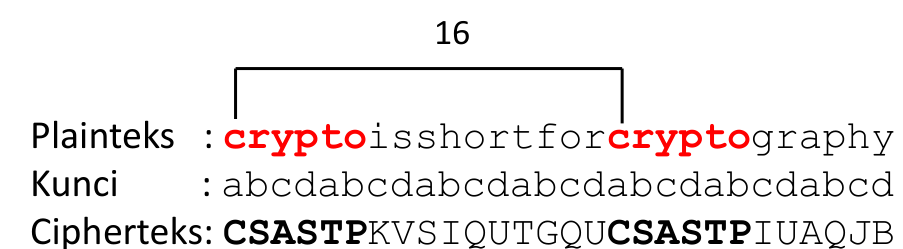
\includegraphics[width=98.70mm,height=68.31mm]{../../images/llm/page_051_img_01.png}%
\end{textblock*}

\end{document}
